\clearpage
\thispagestyle{plain}
\chapter{Results} \label{chap:results}
% \todo[inline]{how to handle suboptimally solved instances}
% \unsure[inline]{font for BiGG, SCIP, ll-FBA etc?}
% \todo[inline]{update label to "ll-FBA", change to latex font, make colors and linestyles consistent over all plots}
% \todo[inline]{subcaptions should explain how to read figure; conclusions and observations are in text}
\todo[inline]{compare solution methods not ll-FBA to CB, both solve ll-FBA}
\todo[inline]{add instances to caption}
% \todo[inline]{update labels in plots}
% \todo[inline]{how to abbreviate MIS \%}
% \todo[inline]{how to refer to original DP}

\todo[inline]{differentiate btw cutting planes and decomposition}
In this section, we present the results of the computational experiments. The performance of solving the big-M reformulation of \textsf{ll-FBA} (\cref{problem:llfba}) directly with \textsf{SCIP} is shown in \cref{section:methods_ll_fba_variants}. We experiment with blocking cycles (\cref{section:results_blocking_cycles}), decomposing the \textsf{ll-FBA} problem (\cref{section:results_cuts}) and the convex-hull formulation (\cref{section:results_dp}).

The code\footnote{available at \\ {\fontsize{9}{48}  \url{https://github.com/hannahtro/Loopless_Fluxes_with_Mixed_Integer_Optimization}}} is written in \textsf{Julia} 1.9.0. We use \textsf{JuMP} \cite{JuMP} and \textsf{MathOptInterface} \cite{mathoptinterface} to build the mathematical models. The MIP solver used in the experiments is \textsf{SCIP}~\cite{SCIP}. The LP solver used is \textsf{HiGHS} \cite{HiGHS}. We use \textsf{COBREXA} \cite{cobrexa} to load the biological model data.
The experiments were carried out on a 64-core compute node equipped with an Intel Xeon Gold 6338 2GHz CPU and 512GB RAM. The CPU memory was limited to 3000MB. 

\section{ll-FBA Variants} \label{section:methods_ll_fba_variants}
First, we look at the performance of solving the different \textsf{ll-FBA} variants by \textsf{SCIP} directly. We compare the running time and number of solved BiGG instances of \textsf{ll-FBA~(indicator)} (\cref{problem:thermo_fba_indicator}), of \textsf{ll-FBA (big-M)} (\cref{problem:thermo_fba_bigM}) and of \mbox{\textsf{ll-FBA (nullspace)} (\cref{problem:llfba_nullspace})}.\\
The results are shown in \cref{fig:ll_fba_comparison}.
We solve around $58\%$ of the \mbox{\textsf{ll-FBA (big-M)}} instances, whereas around $31\%$ of the \textsf{ll-FBA (nullspace)} instances are solved. We solve around $28\%$ of the \textsf{ll-FBA (indicator)} instances. \textsf{iSB619} is infeasible for \mbox{\textsf{ll-FBA (indicator)}} and is therefore excluded from the experiments with indicator constraints. %\todo[inline]{update}

\begin{figure}[h!]
    \centering
    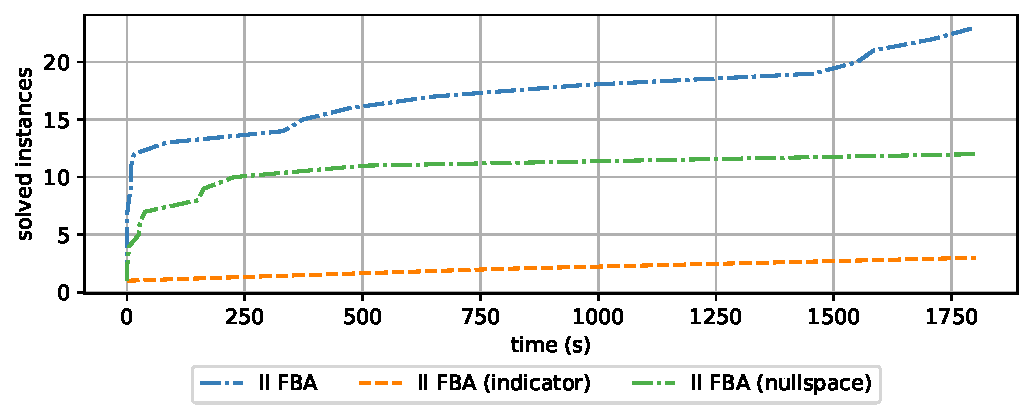
\includegraphics[width=0.983\textwidth]{Images/fba_variants_comparison_plot.pdf}
    \caption{\label{fig:ll_fba_comparison} Performance of the different \textsf{ll-FBA} variants.}
    \subcaption*{Comparing the number of optimally solved BiGG instances of different MIP formulations of \textsf{ll-FBA} within the time limit of 1800 seconds. The variants are solved by \textsf{SCIP} directly. We compare \textsf{ll-FBA (big-M)}, \textsf{ll-FBA (indicator)} and \textsf{ll-FBA (nullspace)}. The plot is based on \cref{tab:ll_fba_comparison} and \cref{tab:ll_fba_indicator}.}
\end{figure}

% ll FBA solves 22 and does not solve 15
\newpage
As we solve twice as many \textsf{ll-FBA (big-M)} instances as \textsf{ll-FBA (nullspace)} instances, we use the \textsf{ll-FBA (big-M)} problem for the other experiments. Even though we also solve fewer \textsf{ll-FBA (indicator)} instances than \textsf{ll-FBA (big-M)} instances, we use the \textsf{ll-FBA (indicator)} for further experiments. Due to the explicit indicator constraints, the solving procedure is different compared to a mixed-integer linear program. With indicator constraints, fewer instances are solved, but some instances are solved much faster. For example, the \textsf{ll-FBA (indicator)} problems of models \textsf{iMM1415} and \textsf{iJN746} are solved in 71 and 10 seconds, whereas with the \textsf{ll-FBA(big-M)} formulations, we need 1550 and 332 seconds (see \cref{tab:ll_fba_comparison}). %\todo[inline]{justify why instances are highlighted}

\section{Blocking Cycles in ll-FBA} \label{section:results_blocking_cycles}
We experiment with blocking cycles in \textsf{ll-FBA (big-M)} as explained on a subset of BiGG instances (see \cref{section:blocking_cycles}).
We then compare solving \textsf{ll-FBA (big-M)} directly to 8 different setups. We block any 10, 20, 50 and 100 cycles, and the 10, 20, 50 and 100 shortest cycles found prior to solving \textsf{ll-FBA (big-M)}. 
We solve each setup with five different \textsf{SCIP} seeds for each model and set the time limit to 1800 minutes. The results are shown in \cref{fig:cff_comparison}.\\
We see that the running time for the models \textsf{e\_coli\_core}, \textsf{iCN900}, \textsf{iAF692} and \textsf{iJR904} is only a few seconds and we see no impact of the different \textsf{SCIP} seeds. Model \textsf{iML1515} cannot be solved within the given time limit by any solving strategy. For the other instances, we observe a small instance variability for \textsf{ll-FBA (big-M)} which shows that the difficulty is consistent across seeds and does not depend on the performance variability of \textsf{SCIP}. The performance of the different solving strategies varies strongly. 
The instance variability of the setups differs significantly. Often, we see hardly any variability, while the running time for others varies up to 10 minutes, for example \textsf{ll-FBA blocked 50} and \textsf{ll-FBA blocked 100} on \textsf{iSFV\_1184}, and for \textsf{ll-FBA shortest blocked 20} and \textsf{ll-FBA shortest blocked 100} on \textsf{iMM904} \todo[inline]{make clearer: I don't quite understand this sentence. A couple of sentences before you said that the instance variability is very small?}. Some instances are solved faster by a blocking cycle strategy than solving \textsf{ll-FBA (big-M)} directly. However, the performance varies for different instances and seeds, and several strategies take much more time and some cannot solve within the time limit.\\
\cref{fig:cff_comparison} is not sufficient to conclude which setup outperforms the other. For such a statement we would require additional tests on more models. 
We also have to consider the time spent in the cycle search, which is not included in the figure (see \cref{tab:cff_time}).
However, the results show that with cuts we can potentially improve the performance compared to solving \textsf{ll-FBA (big-M)} directly, which is tested in detail in the next section.

\begin{figure}[h!]
    \centering
    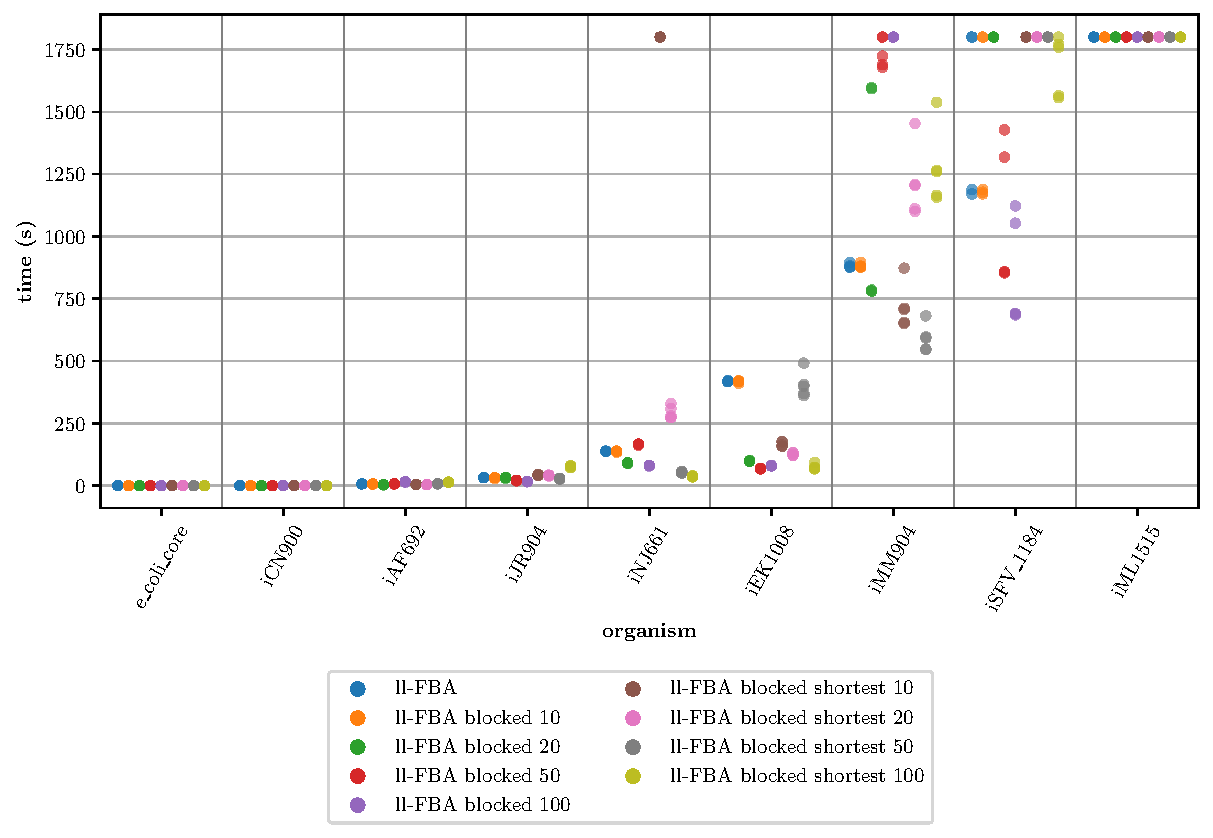
\includegraphics[width=1.0\textwidth]{Images/cff_comparison_boxplot.pdf}
    \caption{Performance of blocking cycle strategies}
    \label{fig:cff_comparison}
    \subcaption*{Comparing the running time of solving \textsf{ll-FBA (big-M)} directly and \textsf{ll-FBA (big-M)} with blocked cycles within the time limit of 1800 seconds. We experiment with blocking at most 10,20,50 and 100 (shortest) cycles. Each setup is tested with 5 different \textsf{SCIP} seeds.}
\end{figure}
\todo[inline]{add big-M to label?}
% \todo[inline]{font too small?}

\newpage
\section{Decomposition} \label{section:results_cuts}
% \todo[inline]{rename and reformulate; reformulation of the problem instead of valid inequalities}
Instead of solving the \textsf{ll-FBA} problem directly, we decompose the problem into a master problem, which is the relaxed \textsf{ll-FBA} problem, and add a cut if a relaxed solution does not satisfy the thermodynamic constraints.\\
% \section{No-Good Cuts}
We first compare solving \textsf{ll-FBA (big-M)} directly to solving the decomposition of \textsf{ll-FBA (big-M)} with no-good cuts (see \cref{section:no_good_cuts}). While we are able to solve around $60\%$ by passing \textsf{ll-FBA (big-M)} directly to \textsf{SCIP}, we solve only $8\%$ with no-good cuts. The \textsf{ll-FBA (big-M)} problem of model \textsf{iAF692} is said to be infeasible with the no-good cut method. If we attempt to solve the instance with a higher precision, the instance cannot be solved within the time limit. \cref{fig:no_good_cuts_comparison_plot} shows the running time and the number of solved instances.
With no-good cuts, we only block one assignment of binary variables $\boldsymbol a$ per iteration, therefore many cuts are required to obtain a loopless solution.

\begin{figure}[h!]
    \centering
    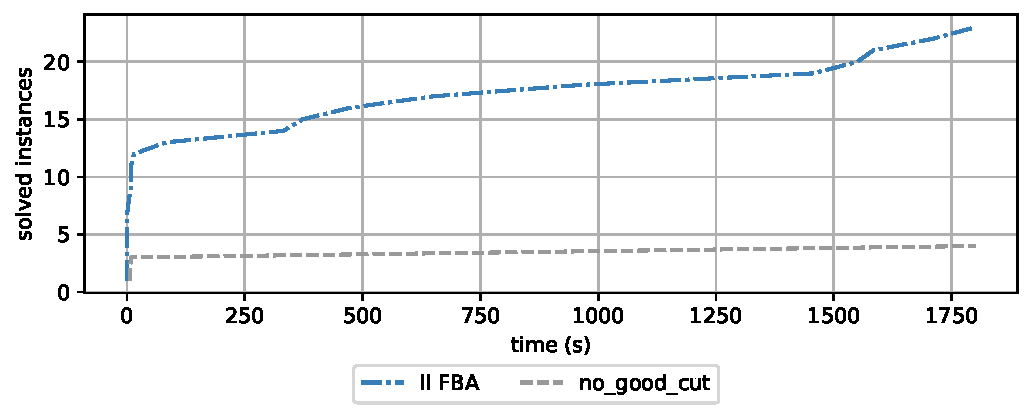
\includegraphics[width=0.983\textwidth]{Images/no_good_cuts_comparison_plot.pdf}
    \caption{Performance of solving the decomposition with no-good cuts}
    \label{fig:no_good_cuts_comparison_plot}
    \subcaption*{Comparing the number of optimally solved BiGG instances solving \textsf{ll-FBA (big-M)} directly and solving the reformulation of \textsf{ll-FBA (big-M)} with no-good cuts within the time limit of 1800 seconds.}
\end{figure}
% \section{Combinatorial Benders' Cuts}

Next, we look at the comparison of the ll-FBA variants with the combinatorial Benders' approach. We experiment with three different formulations of the master problem (\cref{problem:noGoodCut}) and add one cut per iteration of \cref{alg:CB}. We use:
\begin{enumerate}
    \item the indicator formulation, 
    \item the big-M reformulation,
    \item the indicator formulation and big-M reformulation.
\end{enumerate}
\todo[inline]{mention why 3. option makes sense}

\newpage
\cref{fig:comparison_solved_instances_indicator_and_big_m_as_MP} shows the running time and the number of solved BiGG instances by the three combinatorial Benders' setups and by solving \textsf{ll-FBA (big-M)} and \mbox{\textsf{ll-FBA (indicator)}} with \textsf{SCIP} directly within a time limit of 1800 seconds. 
With the combinatorial Benders' approach, we are able to solve many more instances than by solving both ll-FBA variants directly. Combinatorial Benders' cuts are much stronger than no-good cuts. Instead of blocking the entire direction of binary variables $\boldsymbol a$ in the problem, we block one cycle per iteration. \\
Solving \textsf{ll-FBA (indicator)} directly leads to 28\% optimally solved instances, whereas with combinatorial Benders' method with indicator constraints (\textsf{CB (indicator)}) we solve 84\% of the instances to optimality. Solving \textsf{ll-FBA (big-M)} directly leads to 58\% optimally solved instances, whereas with combinatorial Benders' with big-M constraints (\textsf{CB (big-M)}) we solve 92\% of the instances to optimality. %However, \cref{Tab:termination_CB_indicator} and \cref{Tab:termination_CB_big_m} show that for each combinatorial Benders' setup, some instances cannot be solved even though the time limit is not hit. 

\begin{figure}[h!]
    \centering
    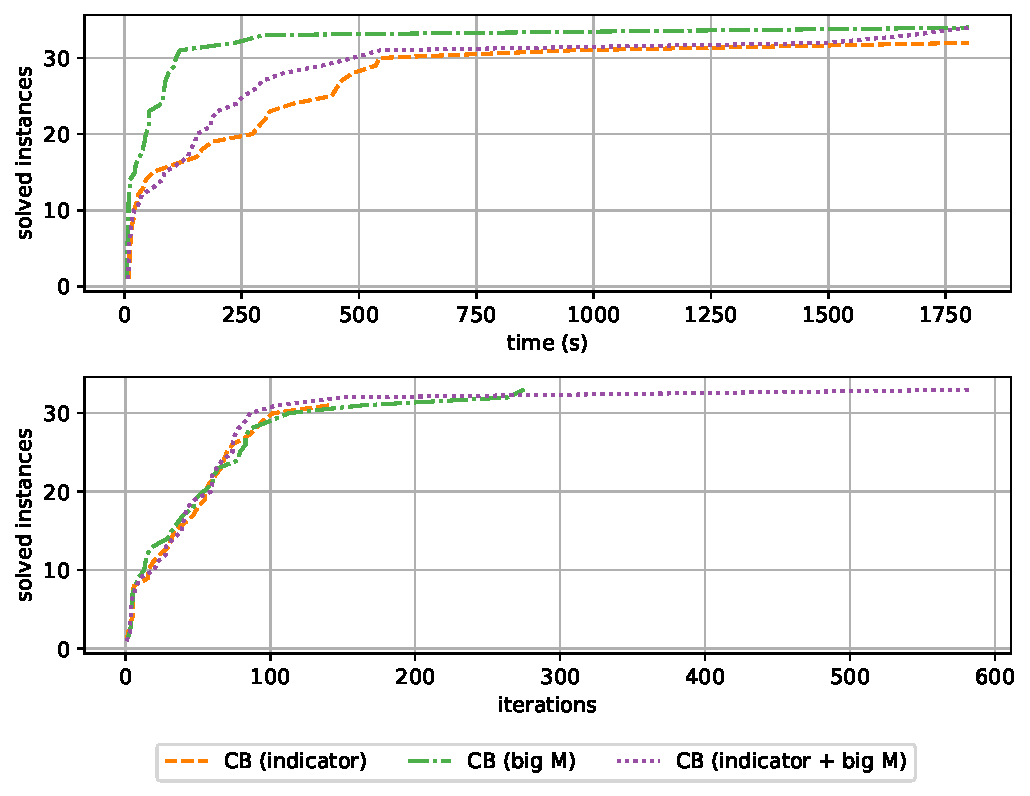
\includegraphics[width=0.983\textwidth]{Images/comparison_solved_instances_indicator_and_big_m.pdf}
    \caption{Performance of CB master problem variants}
    \label{fig:comparison_solved_instances_indicator_and_big_m_as_MP}
    \subcaption*{Comparing the number of optimally solved BiGG instances of \textsf{ll-FBA (big-M)}, \textsf{ll-FBA (indicator)} directly and solving the combinatorial Benders' decomposition of \textsf{ll-FBA} within the time limit of 1800 seconds. We experiment with different formulations of the master problem: big-M reformulation, indicator constraints, and indicator and big-M constraints. Per iteration of the combinatorial Benders' approach, one minimal infeasible subsystem is computed.}
\end{figure}

\newpage
However, \cref{Tab:termination_CB} shows that for the combinatorial Benders' decomposition of \mbox{\textsf{ll-FBA (big-M)}}, one instance is said to be infeasible, even though solving \mbox{\textsf{ll-FBA (big-M)}} returns an optimal solution. If we solve the instance with a tighter tolerance, we find an optimal solution in 264 seconds, whereas solving the \textsf{ll-FBA (big-M)} of \textsf{iRC1080} directly takes 373 seconds.
% \todo[inline]{explain reason for error}
% \todo[inline]{check error}  
\todo[inline]{conclusion for CB variants, mention why indicator+big M not used afterwards}
% \todo[inline]{no good cuts not only block loop but entire flux distribution}

\begin{table}[!ht]
    \centering
    \footnotesize
    \begin{tabular}{@{\extracolsep{4pt}}lllllll@{}}
    \hline
        \multicolumn{2}{c}{} & \multicolumn{2}{c}{\textbf{ll-FBA (indicator)}} & \multicolumn{3}{c}{\thead{CB (indicator)}} \\ \cline{3-4} \cline{5-7} 
        \thead{time (s)} & \thead{\# instances} & \thead{\# optimal} & \thead{\# time \\ limit} & \thead{\# optimal} & \thead{\# time \\ limit} & \thead{\# error} \\ \hline
        0-10 & 10 & 6 & 3 & 9 & 0 & 1 \\
        10-600 & 5 & 3 & 2 & 3 & 2 & 0 \\
        600-1800 & 6 & 1 & 5 & 5 & 1 & 0 \\
        1800-Inf & 15 & 0 & 15 & 13 & 2 & 0 \\
    \end{tabular}

    \begin{tabular}{@{\extracolsep{4pt}}lllllll@{}}
    \hline
        \multicolumn{2}{c}{} & \multicolumn{2}{c}{\textbf{ll-FBA (big-M)}} & \multicolumn{3}{c}{\thead{CB (big-M)}} \\ \cline{3-4} \cline{5-7} 
        \thead{time (s)} & \thead{\# instances} & \thead{\# optimal} & \thead{\# time \\ limit} & \thead{\# optimal} & \thead{\# time \\ limit} & \thead{\# error} \\ \hline
        0-10 & 10 & 10 & 0 & 10 & 0 & 0 \\ 
        10-600 & 5 & 5 & 0 & 4 & 0 & 1 \\ 
        600-1800 & 6 & 6 & 0 & 6 & 0 & 0 \\ 
        1800-Inf & 15 & 0 & 15 & 13 & 2 & 0 \\ \hline
    \end{tabular}
    \caption{\label{Tab:termination_CB} \small Comparing the termination status of solving \textsf{ll-FBA (indicator)} directly and solving \textsf{ll-FBA (indicator)} with the combinatorial Benders' decomposition within a time limit of 1800 seconds (above). Below we compare the termination status of solving \textsf{ll-FBA (big-M)} directly and solving \textsf{ll-FBA (big-M)} with the combinatorial Benders' decomposition. Per iteration of the combinatorial Benders' approach, one minimal infeasible subsystem is computed. The BiGG instances are divided depending on the running time of solving the corresponding ll-FBA variant with \textsf{SCIP} directly.}
\end{table}

So far, we added one combinatorial Benders' cut per iteration of \cref{alg:CB}. In \cref{fig:mis_comparison_solved_instances} we compare the performance of solving \textsf{ll-FBA (indicator)} directly with solving it with the combinatorial Benders' method by experimenting with the number of cuts added per iteration (see \cref{section:cb}). As expected, using more cuts than one per iteration reduces the running time. Any combinatorial Benders' setup with multiple cuts per iteration solves faster than adding a single cut per iteration. For most setups, we see that more cuts lead to fewer iterations. However, too many cuts per iteration can lead to more iterations and a worse overall running time. For example, when blocking up to 20\% of the number of reactions in the model per iteration, the number of iterations increases for some instances and the overall performance is reduced. \\ %\todo[inline]{\% here misleading}
\cref{Tab:termination_mis_indicator} shows that more cuts per iteration affect the termination status marginally. The errored instance corresponds to model \textsf{iSB169} as solving the ll-FBA (indicator) problem directly terminated due to infeasibility. 

\begin{figure}[h!]
    \centering
    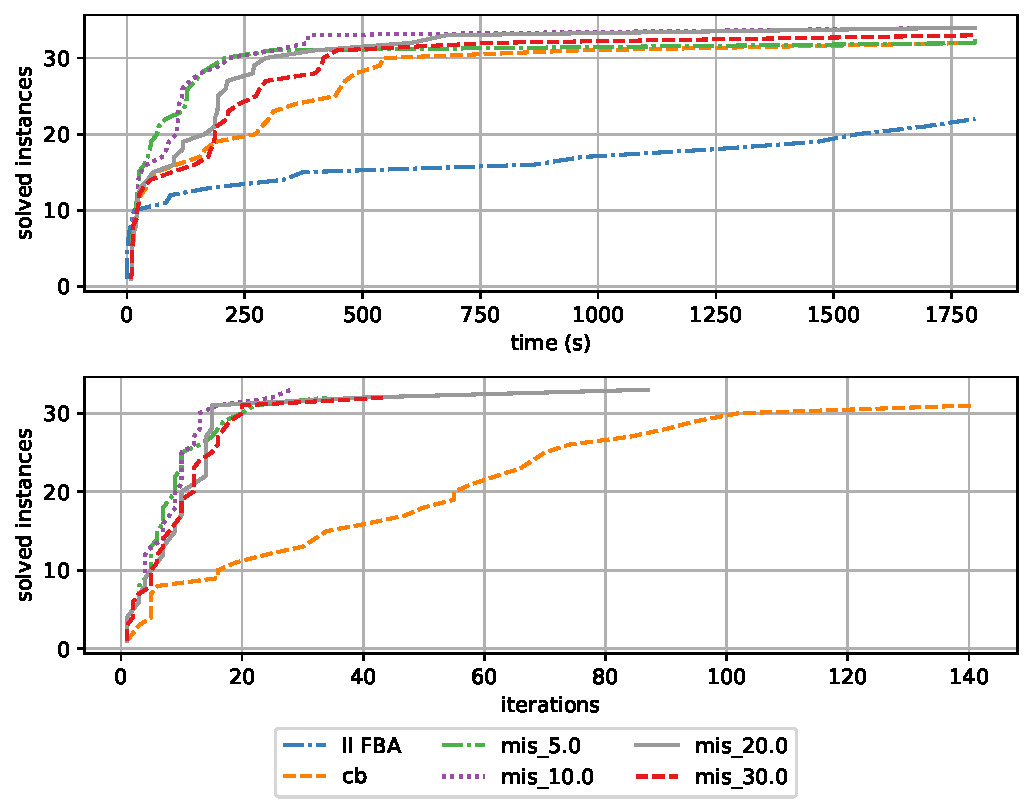
\includegraphics[width=0.983\textwidth]{Images/mis_comparison_solved_instances.pdf}
    \caption{Performance of \textsf{CB (indicator)} with multiple cuts}
    \label{fig:mis_comparison_solved_instances}
    \subcaption*{Comparing the number of optimally solved BiGG instances of solving \textsf{ll-FBA (indicator)} directly and solving the combinatorial Benders' decomposition. We experiment with the number of cuts added per iteration of the combinatorial Benders' approach depending on the instance size. MIS 0.5\% means that at most $k$ cuts are added per iteration, where $k$ is 0.5\% of the number of reactions of the model.}
\end{figure}
% \todo[inline]{extend sentence about MIS; cuts per iteration...}
% \todo[inline]{add less cuts? \\ mention number of cuts per iteration}

\begin{table}[!ht]
    \centering
    \footnotesize
    \begin{tabular}{@{\extracolsep{4pt}}rrrrrr@{}}
    \hline
        \multicolumn{1}{c}{} & \multicolumn{2}{c}{\textbf{ll-FBA (indicator)}} & \multicolumn{3}{c}{\textbf{CB (indicator)}} \\ \cline{2-3} \cline{4-6}
        \thead{MIS \%} & \thead{\# optimal} & \thead{\# time limit} & \thead{\# optimal} & \thead{\# time limit} & \thead{\# error} \\ \hline
        0.1 & 10 & 25 & 31 & 4 & 1 \\ 
        0.5 & 10 & 25 & 32 & 3 & 1 \\
        1.0 & 10 & 25 & 32 & 3 & 1 \\
        2.0 & 10 & 25 & 32 & 3 & 1 \\
        5.0 & 10 & 25 & 32 & 3 & 1 \\
        10.0 & 10 & 25 & 32 & 3 & 1 \\
        20.0 & 10 & 25 & 31 & 4 & 1 \\ \hline       
        % 30.0 & 10 & 25 & 32 & 4 & 1 \\ \hline
    \end{tabular}
    \caption{\label{Tab:termination_mis_indicator}\small Comparing the termination status of solving \textsf{ll-FBA (indicator)} directly and solving \textsf{ll-FBA (indicator)} with the combinatorial Benders' decomposition within a time limit of 1800 seconds. We experiment with the number of cuts added per iteration of the combinatorial Benders' approach. MIS 0.5\% means that at most $k$ cuts are added per iteration, where $k$ is 0.5\% of the number of reactions of the model. The BiGG instances are divided depending on the running time of solving \textsf{ll-FBA (indicator)} with \textsf{SCIP} directly.}
\end{table}
% \todo[inline]{remove iSynC and iSB619 ad they are infeasible for ll-FBA (indicator)}
% \todo[inline]{check instance number, should be 37 or correspond to other table}

\newpage
In \cref{fig:mis_comparison_time_vs_iterations}, we see that with several cuts per iteration, the number of iterations is reduced while the time spent in the MIS search is larger. The average time spent in solving the master problem is smaller but overall much less than the time spent in the MIS search.

\begin{figure}[h!]
    \centering
    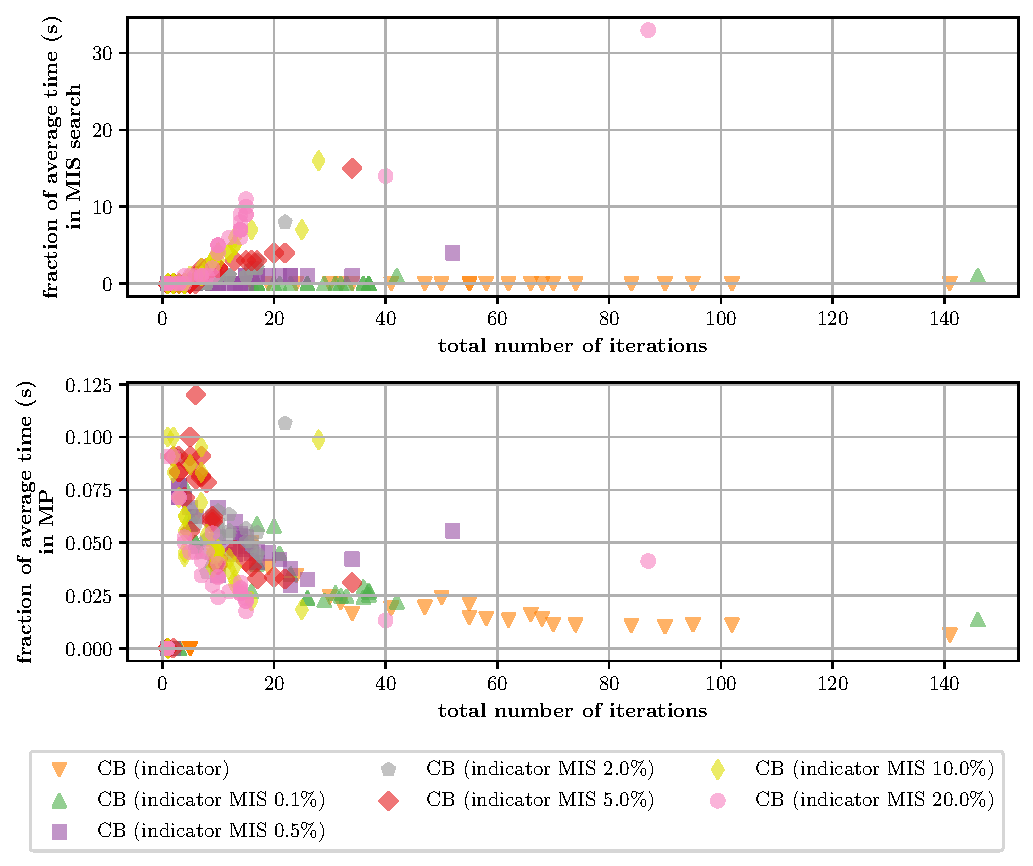
\includegraphics[width=0.983\textwidth]{Images/mis_comparison_time_vs_iterations.pdf}
    \caption{Time spent in master problem (indicator) and in MIS search}
    \label{fig:mis_comparison_time_vs_iterations}
    \subcaption*{We compare the fraction of average time spent in the MIS search of the total running time to the total number of iterations solving \textsf{ll-FBA (indicator)} with the combinatorial Benders' approach on top. Below we compare the fraction of average time spent in the master problem of the total running time to the total number of iterations. We experiment with the number of cuts added per iteration of the combinatorial Benders' approach depending on the instance size. MIS 0.5\% means at most 0.5\% of the number of reactions of the model. We compute the average with the geometric mean. We analyze BiGG instances where solving \textsf{ll-FBA} directly takes more than 15 seconds.}
\end{figure}
\todo[inline]{I don't understand how you get this fraction. Is it solving time vs time limit?}

\clearpage
Next, we compare solving \textsf{ll-FBA (big-M)} directly to solving it with the combinatorial Benders' approach (see \cref{section:cb}) by experimenting with the number of cuts added per iteration. With one cut per iteration, we already solve 92\% of the BiGG instances to optimality and are faster than the combinatorial Benders' decomposition with indicator constraints. As with indicator constraints, with big-M constraints adding multiple cuts per iteration can speed up the solution process. However, adding MIS 2\% or more cuts per iteration performs much worse than combinatorial Benders' with one cut per iteration and fewer iterations are solved within the time limit. With 0.5\% MIS we see the best performance overall and require the least number of iterations per instance.  

\begin{figure}[h!]
    \centering
    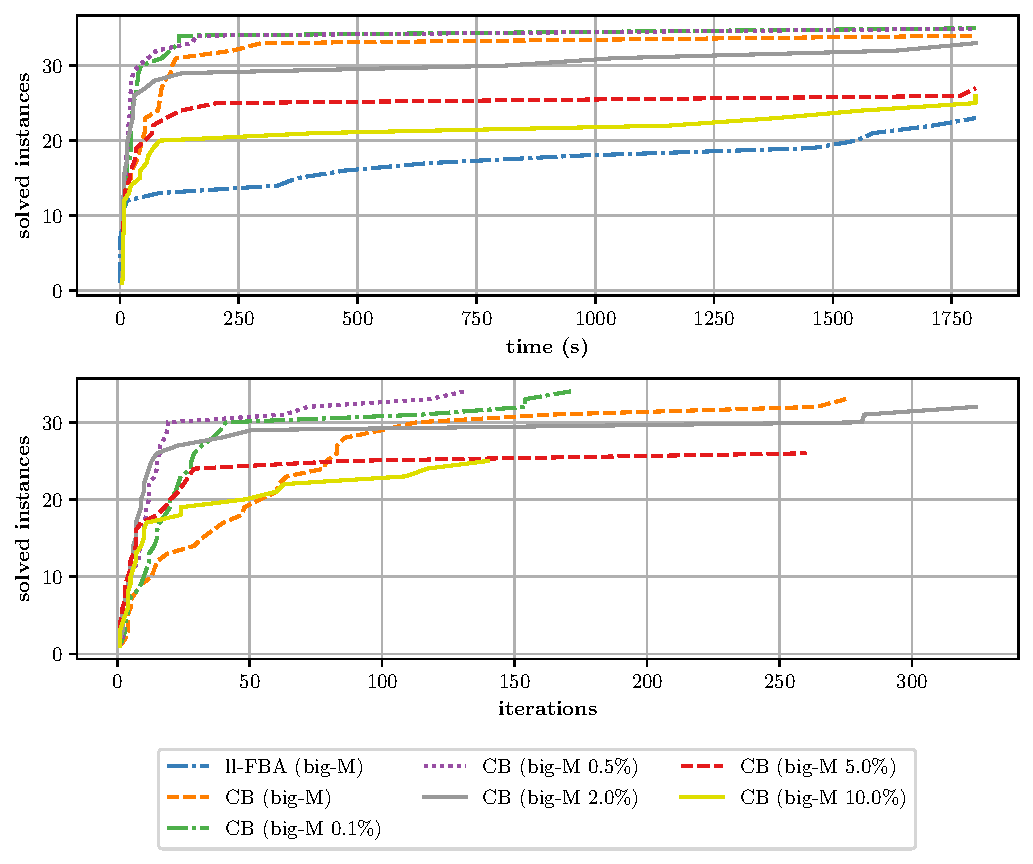
\includegraphics[width=0.983\textwidth]{Images/mis_comparison_solved_instances_big_m.pdf}
    \caption{Performance of \textsf{CB (big-M)} with multiple cuts}
    \label{fig:mis_comparison_solved_instances_big_m}
    \subcaption*{Comparing the number of optimally solved BiGG instances of solving \textsf{ll-FBA (big-M)} directly and solving it with the combinatorial Benders' decomposition within a time limit of 1800 seconds. We experiment with the number of cuts added per iteration of the combinatorial Benders' approach depending on the instance size. MIS 0.5\% means that at most $k$ cuts are added per iteration, where $k$ is 0.5\% of the number of reactions of the model.}
\end{figure}
% \todo[inline]{add less cuts}

\newpage
In \cref{Tab:termination_mis_big_m} we see that with MIS 5.0\% or an MIS 10 \%, we solve significantly fewer instances due to hitting the time limit. The errored instance corresponds to the instance that is said to be infeasible (see \cref{Tab:termination_CB}). With a good choice of allowed cuts per iteration, we outperform the combinatorial Benders' method with indicator constraints. On the other hand, the choice of allowed cuts per iteration can increase the running time significantly in the combinatorial Benders' decomposition with big-M constraints.
% \todo[inline]{rephrase robust: On the other hand, the choice of allowed cuts can impact the running time more negatively compared to indicator constraint formulation.}.

\begin{table}[!ht]
    \centering
    \footnotesize
    \begin{tabular}{@{\extracolsep{4pt}}rrrrrr@{}}
    \hline
        \multicolumn{1}{c}{} & \multicolumn{2}{c}{\textbf{ll-FBA (big-M)}} & \multicolumn{3}{c}{\textbf{CB (big-M)}} \\ \cline{2-3} \cline{4-6}
        \thead{MIS \%} & \thead{\# optimal} & \thead{\# time limit} & \thead{\# optimal} & \thead{\# time limit} & \thead{\# error} \\ \hline
        0.1 & 21 & 15 & 32 & 3 & 1 \\
        0.5 & 21 & 15 & 32 & 3 & 1 \\
        1.0 & 21 & 15 & 32 & 3 & 1 \\
        2.0 & 21 & 15 & 31 & 4 & 1 \\
        5.0 & 21 & 15 & 26 & 9 & 1 \\
        10.0 & 21 & 15 & 24 & 11 & 1 \\ \hline
        % 20.0 & 22 & 15 & 20 & 15 & 2 \\
        % 30.0 & 22 & 15 & 20 & 14 & 3 \\ \hline
    \end{tabular}
    \caption{\label{Tab:termination_mis_big_m}\small Comparing the termination status of solving \textsf{ll-FBA (big-M)} directly and solving \textsf{ll-FBA (big-M)} with the combinatorial Benders' method on the BiGG instances within a time limit of 1800 seconds. We experiment with the number of cuts added per iteration of the combinatorial Benders' approach depending on the instance size. MIS 0.5\% means that at most $k$ cuts are added per iteration, where $k$ is 0.5\% of the number of reactions of the model.}
\end{table}

The comparison of the fraction of average time spent in the MIS search and in the master problem with big-M constraints in relation to the total number of iterations is less structured than the comparison with the indicator setting. Overall, the time spent in the MIS search and in solving the master problem is larger with more cuts, however, fewer iterations are to solve.

\begin{figure}[h!]
    \centering
    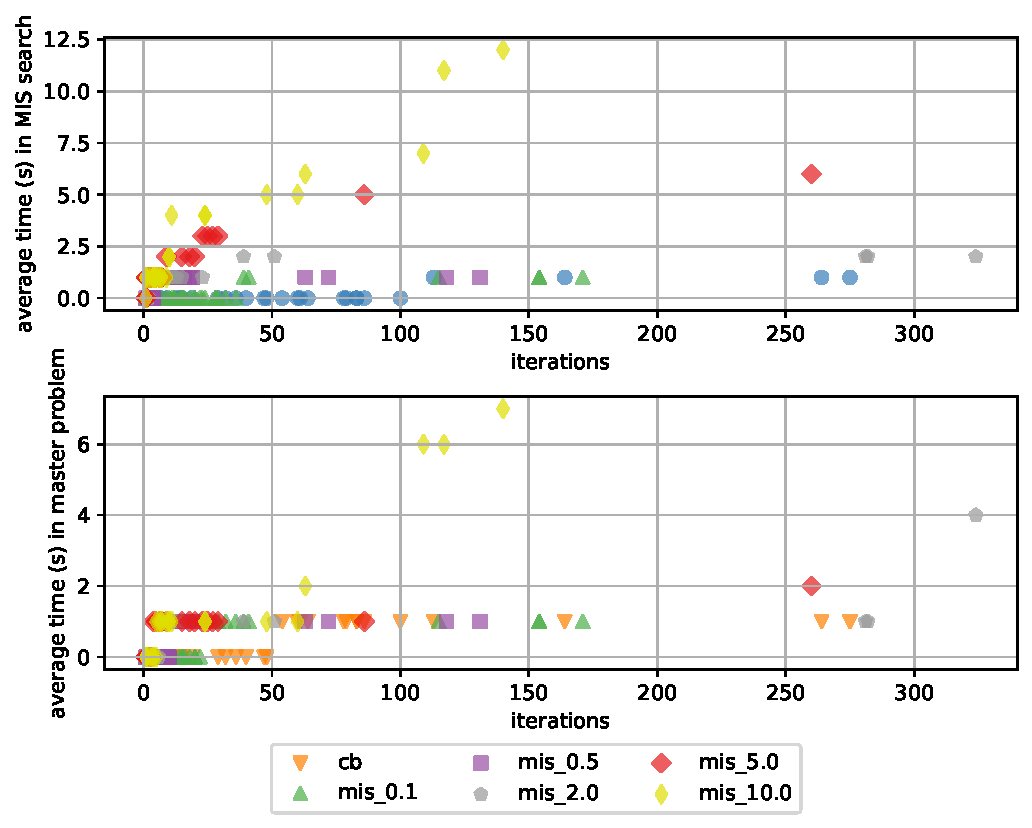
\includegraphics[width=0.983\textwidth]{Images/mis_comparison_time_vs_iterations_big_m.pdf}
    \caption{Time spent in master problem (big-M) and MIS search}
    \label{fig:mis_comparison_time_vs_iterations_big_m}
    \subcaption*{We compare the fraction of average time spent in the MIS search of the total running time to the total number of iterations of solving \textsf{ll-FBA (big-M)} with the combinatorial Benders' decomposition on top. Below we compare the fraction of average time spent in the master problem of the total running time to the total number of iterations. We experiment with the number of cuts added per iteration of the combinatorial Benders' method depending on the instance size. MIS 0.5\% means that at most $k$ cuts are added per iteration, where $k$ is 0.5\% of the number of reactions of the model. We compute the average with the geometric mean. We analyze BiGG instances where solving \textsf{ll-FBA} directly takes more than 15 seconds.}
\end{figure}

Instead of using \textsf{JuMP} to build the master problem, which builds a model in every iteration, we experiment with using a constraint handler in \textsf{SCIP} directly. Even though using a constraint handler should decrease the running time as the model is reused throughout the solving procedure, we do not see a better performance in preliminary experiments (see \cref{Tab:ch_vs_cb}). We therefore continue with building the models in \textsf{JuMP}.

After experimenting with several formulations of the master problem and with the number of cuts per iteration of \cref{alg:CB}, we test both solving strategies on the yeast models (see \cref{section:methods_yeast}), which are larger than most BiGG models tested. In \cref{Tab:yeast}, we see that neither solving strategy performs well on the yeast instances. \todo[inline]{some discussion on this? What are possible reasons/aspects (while acknowledging that it is difficult to pin down why this failed), maybe 1-2 sentences. Maybe this could be connected to the Conclusion as an outloo} Only with one strategy we solve 1 out of 11 instances. On one yeast instance, we terminate due to an error on \textsf{SCIP}: the maximal depth level is exceeded even though it is set to 100,000.

% In comparison to the BiGG models tested, combinatorial Benders with big-M constraints is more robust. Combinatorial Benders with indicator constraints leads to more errors in the solution process. 

\begin{table}[!ht]
    \centering
    \footnotesize
    \begin{tabular}{@{\extracolsep{4pt}}lrrr@{}}
        \hline
        \thead{solving strategy} & \thead{\# optimal} & \thead{\# time limit} & \thead{\# error} \\ \hline
        ll-FBA (big-M) & 0 & 11 & 0 \\
        CB (big-M) & 0 & 11 & 0 \\
        CB (indicator) & 0 & 11 & 0 \\
        CB (big-M MIS 0.1 \%) & 0 & 11 & 0 \\
        CB (big-M MIS 0.2 \%) & 0 & 11 & 0 \\
        CB (big-M MIS 0.5 \%) & 1 & 10 & 0 \\
        CB (big-M MIS 2.0 \%) & 0 & 11 & 0 \\
        CB (indicator MIS 0.1 \%) & 0 & 11 & 0 \\
        CB (indicator MIS 0.2 \%) & 0 & 11 & 0 \\
        CB (indicator MIS 0.5 \%) & 0 & 11 & 0 \\
        CB (indicator MIS 2.0 \%) & 0 & 10 & 1 \\ \hline
    \end{tabular}
    \caption{\label{Tab:yeast}\small Comparing the termination status of solving yeast instances with \textsf{ll-FBA (big-M)}  directly and solving \textsf{ll-FBA (big-M)} with the combinatorial Benders' method within a time limit of 1800 seconds. We experiment with different formulations of the master problem: indicator constraints, and big-M constraints. We compare adding a single cut per iteration of the combinatorial Benders' method denoted by \textsf{CB} and adding multiple cuts. MIS 0.5\% means that at most $k$ cuts are added per iteration, where $k$ is 0.5\% of the number of reactions of the model.}
\end{table}
% \todo[inline]{combinatorial Benders' iteration correct?}

\newpage
Finally, we experiment with solving enzyme models with the combinatorial Benders' approach. We compare solving \textsf{ll-FBA (big-M)} directly to solving it with the combinatorial Benders' decomposition, as the big-M formulation showed the best performance on the other experiments. We compare blocking one cycle per iteration to blocking $k$ cycles per iteration, where $k$ is 0.5\% of the number of reactions of the model. The results are shown in \cref{fig:comparison_gecko}.
We see that both combinatorial Benders' variants solve similarly and outperform solving \textsf{ll-FBA (big-M)} directly. Both combinatorial Benders' variants require few iterations for most instances. As the reaction rate is limited by enzyme abundance, the relaxed solution contains already fewer loops. Therefore, less cuts are needed to obtain an optimal solution.
\vspace*{-\baselineskip}

\begin{figure}[h!]
    \centering
    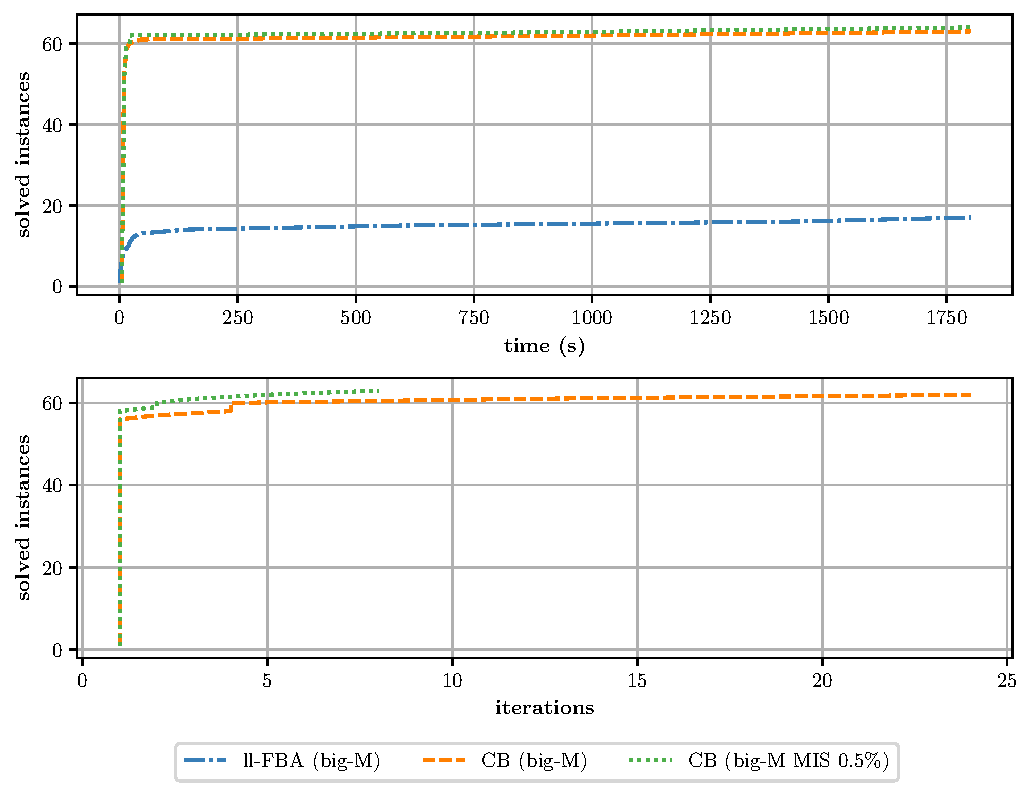
\includegraphics[width=0.983\textwidth]{Images/comparison_solved_instances_gecko_1.0e-8.pdf}
    \caption{\label{fig:comparison_gecko} Performance of the combinatorial Benders' method on enzyme models}
    \subcaption*{Comparing the number of optimally solved instances with enzyme constraints of solving \textsf{ll-FBA (big-M)} directly, and solving the problem with the combinatorial Benders' approach within the time limit of 1800 seconds. We experiment with adding a single cut per iteration of the combinatorial Benders' approach and with adding at most $k$ cuts per iteration, where $k$ is 0.5\% of the number of reactions in the model.}
\end{figure}

\newpage
However, looking at \cref{Tab:gecko}, we see that the combinatorial Benders' approach is not stable. We solve around 70\% of instances to optimality but terminate the solution process in 18\% of the instances not due to time limit but due to errors in the solving process. The enzyme models are numerically challenging. The majority of errors are due to an assertion to ensure that the objective value of the master problem in the first iteration is equal to the objective problem of the \textsf{FBA} problem within a tolerance of $1e-3$. In other instances, we cannot solve the subproblem due to numeric problems.

\begin{table}[!ht]
    \centering
    \footnotesize
    \begin{tabular}{lrrr}
    \hline
        \thead{solving strategy} & \thead{\# optimal} & \thead{\# time limit} & \thead{\# error} \\ \hline
        ll-FBA (big-M) & 16 & 74 & 0 \\
        CB (big-M) & 63 & 5 & 22 \\
        CB (big-M MIS 0.5 \%) & 64 & 4 & 22 \\ \hline
    \end{tabular}
    \caption{\label{Tab:gecko}\small Comparing the termination status of instances with enzyme constraints of solving \textsf{ll-FBA (big-M)} directly, and solving the problem with the combinatorial Benders' method within the time limit of 1800 seconds. We experiment with adding one cut per iteration of the combinatorial Benders' method and with adding at most $k$ cuts per iteration, where $k$ is 0.5\% of the number of reactions in the model.}
\end{table}

In our case, we are able to solve most enzyme instances within a few seconds. As the enzyme data is randomly generated, we do not make a claim on the performance on enzyme models in general. However, this shows the flexibility of the combinatorial Benders' approach, which can be extended by linear constraints easily.

\newpage
% \section{Intersection Cuts}
\section{Convex-Hull Formulation} \label{section:results_dp}
We have seen that with cuts it is possible to reduce the running time of solving \textsf{ll-FBA (indicator)} and \textsf{ll-FBA (big-M)}. Now we return to the disjunctive programming formulation of our problem. We use the \textsf{DisjunctiveProgramming} package to get the hull formulation and the big-M reformulation. We compare the performance of solving \textsf{ll-FBA (big-M)} directly, solving the big-M reformulation of the disjunctive program with optimizing the choice of $M$, the hull formulation of the disjunctive program and solving \textsf{ll-FBA (big-M)} with combinatorial Benders' cuts within a time limit of 1800 seconds. The difference between our big-M formulation is that in the package the choice of $M$ is optimized. \\
\cref{fig:dp_performance} shows that we solve the least instances with the convex-hull formulation.  
Even though the feasible region of the hull reformulation is the convex hull, the reformulation requires more constraints and decision variables, which leads to an increased running time. With the big-M reformulation of the \textsf{DisjunctiveProgramming} package, we solve more instances than with our big-M formulation. The $M$ constant determines how large the approximation of the feasible region is. Choosing the smallest $M$ possible, we obtain a tighter approximation and more instances can be solved within the time limit. When we compare solving the MIP reformulations to solving \textsf{ll-FBA (big-M)} with combinatorial Benders' cuts, we see that with the latter we are able to solve most of the instances and are significantly faster.

\begin{figure}[h!]
    \centering
    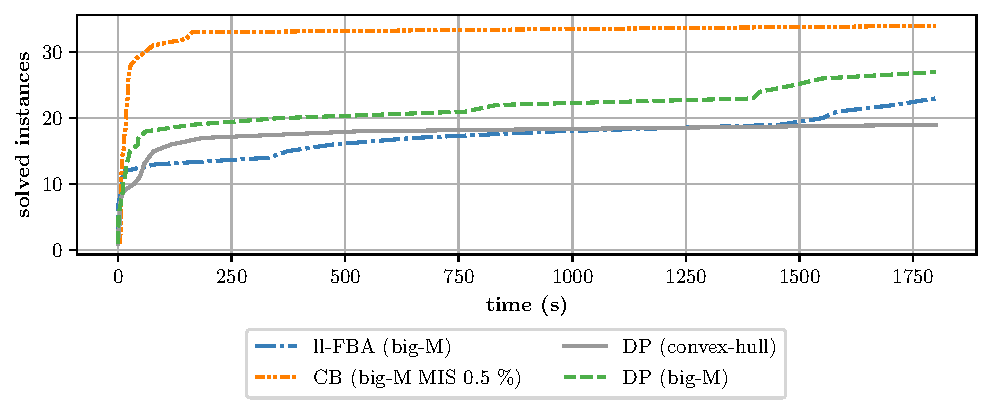
\includegraphics[width=1.0\textwidth]{Images/comparison_dp.pdf}
    \caption{\label{fig:dp_performance} Performance of the big-M reformulation and the convex-hull formulation}
    \subcaption*{Comparing the number of optimally solved BiGG instances of solving \textsf{ll-FBA (big-M)} directly, solving the convex-hull formulation (\textsf{DP (convex-hull)}), solving the big-M formulation of the \textsf{DisjunctiveProgramming} package with optimized $M$ constant (\textsf{DP (big-M)}), and solving the problem with the combinatorial Benders' decomposition (\textsf{CB (big-M MIS 0.5 \%)}) within the time limit of 1800 seconds.}
\end{figure}

% \todo[inline]{instances with smaller objective value are considered as NOT SOLVED, update plot}
% \todo[inline]{add table?}
% \todo[inline]{move dp section to ll-FBA variants?}